\documentclass[border=10pt]{standalone}

\usepackage{tikz}
\usepackage{tikzsymbols}
\usetikzlibrary{calc,patterns,shapes.geometric}

\def\centerarc[#1](#2)(#3:#4:#5){\draw[#1] ($(#2)+({#5*cos(#3)},{#5*sin(#3)})$) arc (#3:#4:#5);}

\begin{document}
	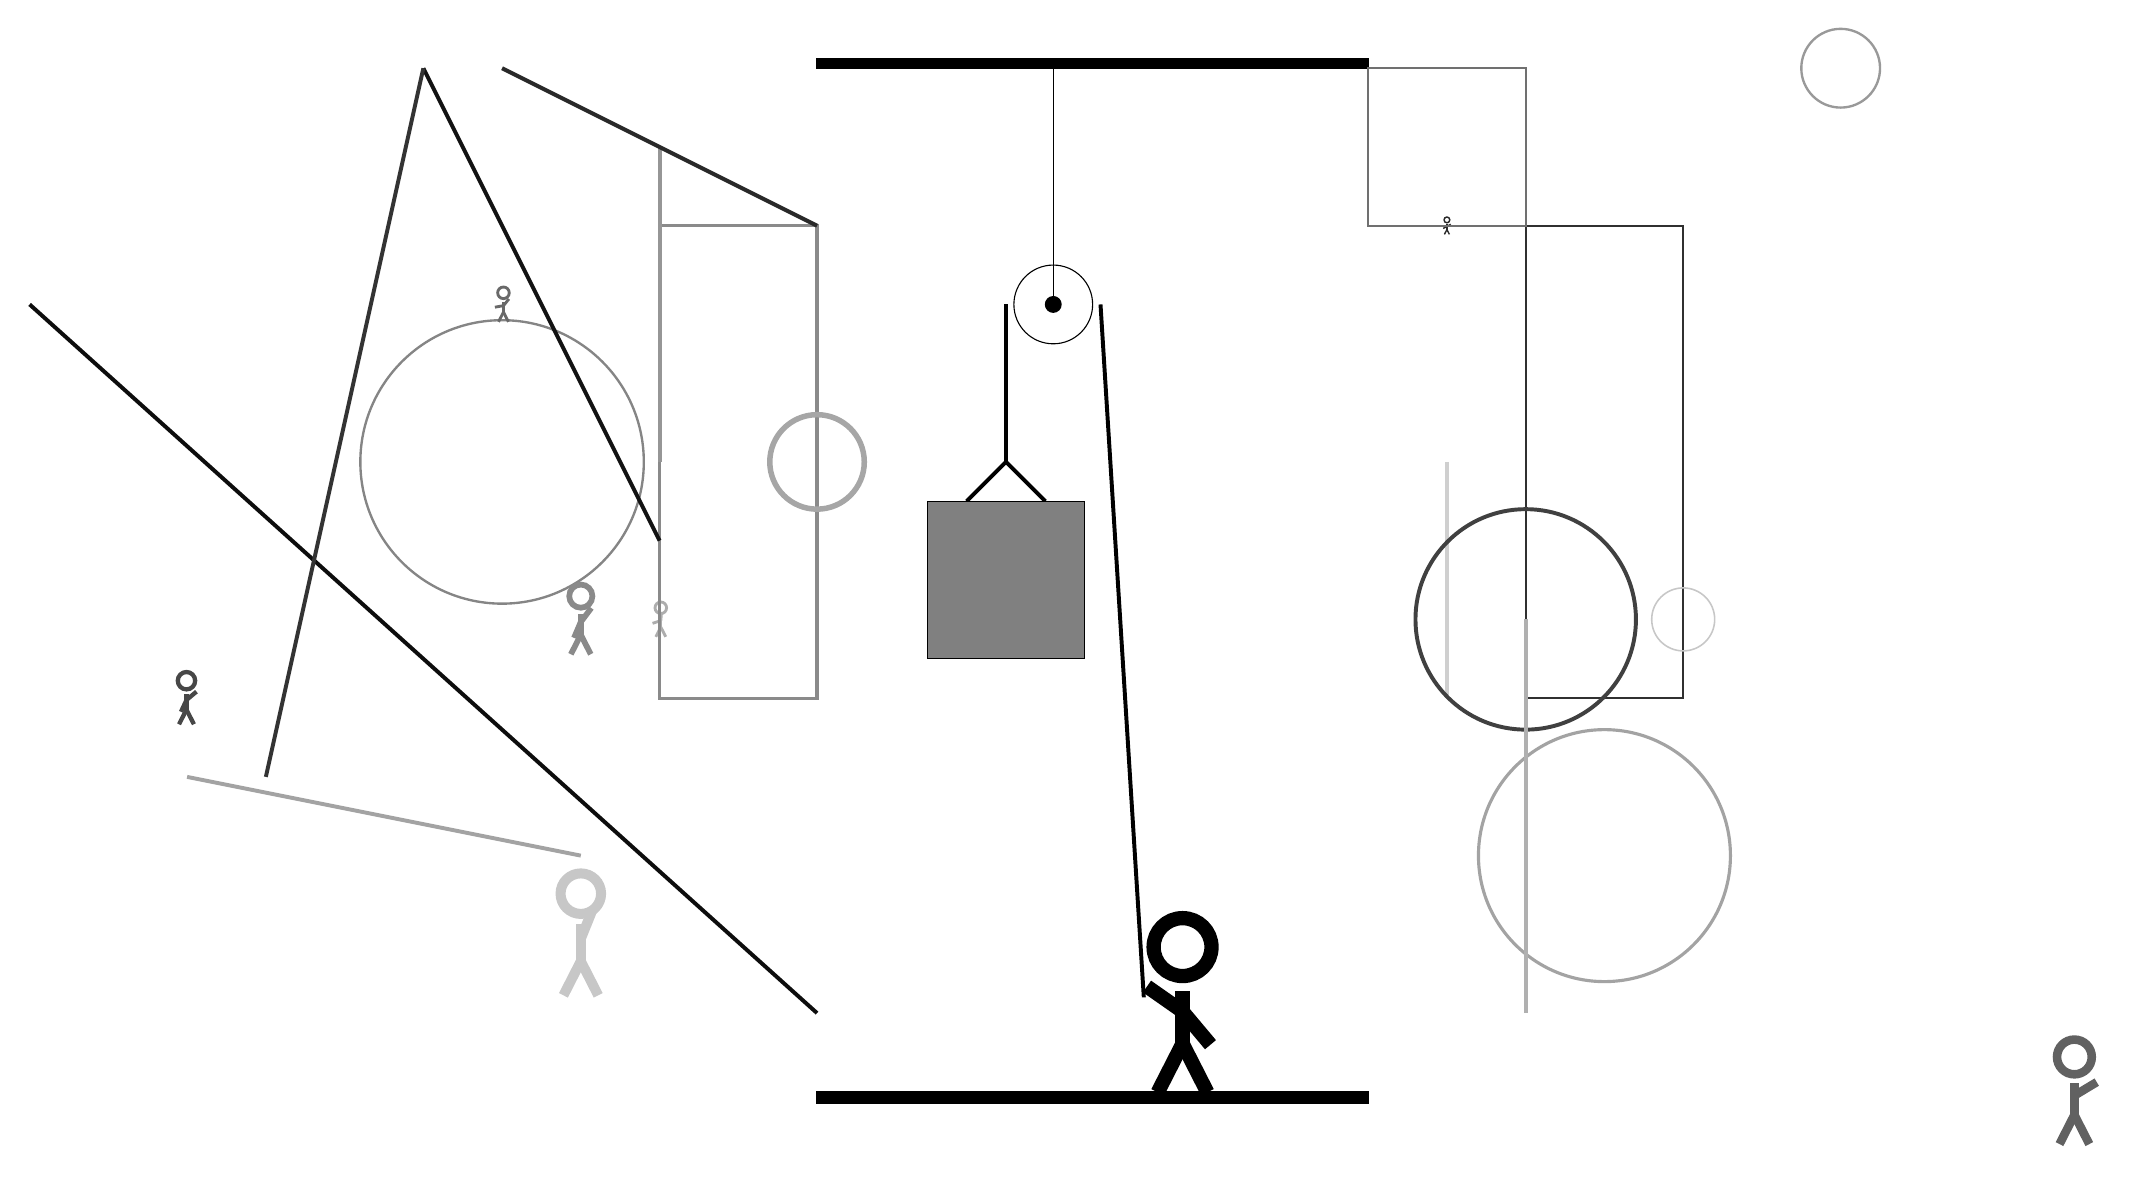
\begin{tikzpicture}
		%%%%% START %%%%%
		
		\draw[fill=black] (-2, 10) rectangle (5, 10.125);
		
		\draw (1, 7) circle (0.5);
		\draw[fill=black] (1, 7) circle (0.1);
		\draw (1, 10) -- (1, 7);
		
		\draw [line width=0.3mm, color=black!48](-6, 5) circle (1.8);
		
		\draw[line width=0.3mm, color=black!81] (7, 2) rectangle (9, 8);
		\node[line width=0.2mm, color=black!59] at (-6, 7) {\Strichmaxerl[2][10][51]};
		\draw[line width=0.5mm, color=black!19](6, 5) -- (6, 2);
		
		\node[line width=0.6mm, color=black!32] at (-4, 3) {\Strichmaxerl[2][18][85]};
		
		\node[line width=0.3mm, color=black!62] at (14, -3) {\Strichmaxerl[6][90][31]};
		\draw[line width=0.4mm, color=black!46] (-4, 8) rectangle (-2, 2);
		
		\draw [line width=0.5mm, color=black!75](7, 3) circle (1.4);
		\draw[line width=0.5mm, color=black!41](-4, 9) -- (-4, 5);
		
		\node[line width=0.4mm, color=black!22] at (-5, -1) {\Strichmaxerl[7][90][68]};
		\draw [line width=0.3mm, color=black!40](11, 10) circle (0.5);
		
		\draw[line width=0.5mm, color=black!93](-4, 4) -- (-7, 10);
		\draw[line width=0.5mm, color=black!84](-2, 8) -- (-6, 10);
		
		\node[line width=0.4mm, color=black!72] at (-10, 2) {\Strichmaxerl[3][65][40]};
		\node[line width=0.3mm, color=black!84] at (6, 8) {\Strichmaxerl[1][30][28]};
		\draw [line width=0.7mm, color=black!35](-2, 5) circle (0.6);
		
		\draw[line width=0.5mm, color=black!95](-2, -2) -- (-12, 7);
		
		\draw[line width=0.5mm, color=black!36](-5, 0) -- (-10, 1);
		\draw [line width=0.4mm, color=black!36](8, 0) circle (1.6);
		\draw[line width=0.3mm, color=black!56] (5, 10) rectangle (7, 8);
		\node[line width=0.3mm, color=black!46] at (-5, 3) {\Strichmaxerl[4][67][53]};
		
		\draw [line width=0.2mm, color=black!22](9, 3) circle (0.4);
		
		\draw[line width=0.5mm, color=black!80](-7, 10) -- (-9, 1);
		\draw[line width=0.5mm, color=black!31](7, 3) -- (7, -2);
		
		\draw[line width=0.5mm] (-0.1, 4.5) -- (0.4, 5.0) -- (0.9, 4.5);
		\draw[fill=black!50] (-0.6, 4.5) rectangle (1.4, 2.5);
		
		\draw[line width=0.5mm] (0.4, 7) -- (0.4, 5.0);
		\centerarc[line width=0.5mm](1, 7)(0:180:0.6);
		\draw[line width=0.5mm](1.6, 7) -- (2.15, -1.8);
		
		\node at (2.6, -1.9) {\Strichmaxerl[10][-35][-50]};
		
		\draw[fill=black] (-2, -3) rectangle (5, -3.15);
		
		%%%%% END %%%%%
	\end{tikzpicture}
\end{document}